% !TEX root = ../main.tex
% =====================================================================
% APPENDIX -- after the references, and clearly marked. Everything here
% supports the main text; nothing here is needed to follow the argument.
%
% Order follows the order a reader would look things up:
%   A metrics, B model and training detail, C additional results.
% =====================================================================

\section{Metric definitions}
\label{app:metrics}

\paragraph{AOPCR.}
Let $\bagpred^{\,c}(\bag)$ be the logit of the predicted class $c$ on the unperturbed series, and let
$\bag^{(m)}$ be the series with the $m$ time steps that the model itself ranks most important for $c$
replaced by the per-series mean. AOPCR integrates the drop over the perturbation order,
\begin{equation}
  \mathrm{AOPCR} = \frac{1}{M+1}\sum_{m=0}^{M}
      \Big( \bagpred^{\,c}(\bag) - \bagpred^{\,c}\big(\bag^{(m)}\big) \Big),
  \label{eq:aopc}
\end{equation}
following \citet{samek2017aopc} as adapted to time series by \citet{early2024millet}, with $M$ set to
$10\,\%$ of the series length in steps of $1\,\%$. Higher is better. Note that \Cref{eq:aopc} is a
difference of \emph{unnormalised} logits, which is the origin of the comparability problem documented
in \Cref{sec:res:aopcr}: two models whose logits live on different scales produce AOPCR values on
different scales, whatever the quality of their rankings.

\paragraph{\ndcg{}.}
Where per-time-step ground truth exists, we instead rank the $\nsteps$ time steps by the claimed
importance $\interp_{c,j}$ and score that ranking with normalised discounted cumulative gain
\citep{jarvelin2002ndcg} at cut-off $n$, the number of steps the generator actually marked as
carrying the class signal. Relevance is binary. The normalisation is against the ideal ranking of the
same series, so \ndcg{} lies in $[0,1]$ and is comparable between models, datasets and papers ---
which is why the interpretation claims of this paper rest on it and not on AOPCR.

\section{Model and training detail}

\subsection{Encoder variants}
\label{app:encoders}

The main text uses two encoders: the plain multi-scale separable stack of \Cref{sec:method:enc}
(\texttt{sea\_mstcn\_sep}) and its bottlenecked form (\Cref{eq:bottleneck},
\texttt{sea\_mstcn\_sep\_bottleneck}). Five further variants were swept and appear in
\Cref{tab:app_encoders}: \emph{gated}, which collapses the time axis to a summary vector and
re-weights channels by it; \emph{input-gated}, which reads the same gate from the raw input instead;
\emph{spike/trend}, which runs a smoothed and a high-pass branch and mixes them;
\emph{reconstruction-residual}, which appends features built from a reconstruction error; and two
\emph{wrappers} that do not replace an encoder but sit around one --- \emph{multi-scale channels},
which adds rolling max/min/std input channels, and \emph{multi-scale pyramid}, which runs the same
encoder at four downsampling rates and fuses back to length $\nsteps$. All preserve $\nsteps$. Only
the bottleneck is part of this paper's contribution; the others are the context showing that the
bottleneck was the right place to cut.

\begin{table}[h]
\caption{Encoder axis: mean over every head the encoder was paired with, \webtraffic{}. $n$ is the
number of pairings. These are means over heterogeneous pairings, so they indicate spread, not a
ranking of encoders.}
\label{tab:app_encoders}
\begin{center}
\small
\begin{tabular}{lcccr}
\toprule
\textbf{Encoder} & Acc. & AOPCR & \ndcg{} & $n$ \\
\midrule
multi-scale channels (wrapper)   & 0.937 & 2.385 & 0.747 & 4 \\
reconstruction-residual          & 0.924 & 2.315 & 0.719 & 5 \\
input-gated                      & 0.904 & 2.345 & 0.718 & 5 \\
gated                            & 0.902 & 2.056 & 0.710 & 19 \\
plain (\texttt{sea\_mstcn\_sep}) & 0.898 & 1.933 & 0.694 & 12 \\
bottleneck                       & 0.884 & 2.209 & 0.694 & 8 \\
spike/trend                      & 0.858 & 1.814 & 0.677 & 7 \\
multi-scale pyramid (wrapper)    & 0.771 & 1.394 & 0.604 & 3 \\
\bottomrule
\end{tabular}
\end{center}
\end{table}

\subsection{Pooling heads}
\label{app:heads}

Every head keeps the two-branch template of \Cref{eq:conj_gate}, so a head is fully described by two
choices: the shape of the attention branch, and the operator that reduces the $\nsteps$ evidence
values $g_j^k$ to one number. \Cref{tab:app_heads} lays out all seven on those two axes together with
the parameter setting at which each becomes conjunctive pooling exactly. Two are adapted from
histopathology MIL rather than designed here: gated attention is due to \citet{ilse2018attention} and
the dual-stream mechanism to \citet{li2021dsmil}; our changes to those two are the transfer to time
series, the per-class formulation, and --- for the dual stream --- removing its contrastive
pre-training and adding a learnable blend.

\begin{table}[h]
\caption{The seven heads as two independent slots. ``Reduces at'' names the setting at which the head
becomes conjunctive pooling exactly. L1--L3 are the limitations listed in \Cref{sec:method:mil}.}
\label{tab:app_heads}
\begin{center}
\scriptsize
\setlength{\tabcolsep}{3.5pt}
\begin{tabular}{lllcc}
\toprule
\textbf{Head} & \textbf{Attention} & \textbf{Reduction over time} & \textbf{Reduces at} & \textbf{Targets} \\
\midrule
Conjunctive (baseline)    & shared gate    & mean                            & --- & --- \\
Class-wise conjunctive    & per-class gate & mean                            & $a_j^k = a_j$ & L1 \\
Softmax conjunctive       & per-class score& softmax, learnable $\tau$       & $\tau \to \infty$ & L2 \\
Adaptive class-wise       & per-class gate & soft-argmax, learnable $\beta_k$& $\beta_k \to 0$ & L3 \\
Top-$k$ conjunctive       & per-class gate & mean of the $k$ largest         & $\kappa = 1$ & L3 \\
Attention-max             & per-class gate & blend of mean and max           & $\lambda_k \to 0$ & L3 \\
Per-class gated attention & gated $\tanh\!\odot\!\sig$ & softmax             & \textbf{none} & L1, L3 \\
Dual-stream conjunctive   & gate $+$ critical query & blend of two streams   & $\lambda \to 0$ & L3 \\
\bottomrule
\end{tabular}
\end{center}
\end{table}

\Cref{tab:app_pooling} averages each head over every encoder it was paired with. Two observations
support statements made in the main text. First, the spread of the head choice ($0.744$ to $0.921$)
is as large as the spread of the encoder choice in \Cref{tab:app_encoders} ($0.771$ to $0.937$), so
the pooling head is a first-class design axis and not a detail. Second, a reduction property is
\emph{not} a safety guarantee: five of the seven heads provably contain conjunctive pooling as a
special case, and the dual-stream head, which is one of them, is nevertheless the worst head tested
--- its four pairings score $0.860$, $0.824$, $0.736$ and $0.556$. The mechanism is visible in the
training runs: its blend weight starts at $\lambda_0 = 0.05$ and nothing in \Cref{eq:loss} pushes it
back towards the reduction point, so being \emph{able} to recover the baseline does not mean being
optimised towards it. That is why the main text argues for \mbox{Top-$k$} on measured \ndcg{} rather
than on its reduction property alone.

\begin{table}[h]
\caption{Head axis: mean over every encoder the head was paired with, \webtraffic{}. Excludes the
$\kappa$ and $\lambda_{\mathrm{focus}}$ ablation configurations and the published-recipe baseline,
which would otherwise weight \mbox{Top-$k$} and the bottleneck encoder.}
\label{tab:app_pooling}
\begin{center}
\small
\begin{tabular}{lcccr}
\toprule
\textbf{Head} & Acc. & AOPCR & \ndcg{} & $n$ \\
\midrule
Class-wise conjunctive    & 0.921 & 2.322 & 0.692 & 10 \\
Per-class gated attention & 0.918 & 1.869 & 0.733 & 4 \\
Adaptive class-wise       & 0.912 & 2.210 & 0.732 & 9 \\
Softmax conjunctive       & 0.907 & 1.690 & 0.712 & 9 \\
Top-$k$ conjunctive       & 0.904 & 2.267 & 0.712 & 16 \\
Attention-max             & 0.838 & 1.758 & 0.645 & 8 \\
Dual-stream conjunctive   & 0.744 & 2.007 & 0.636 & 4 \\
\bottomrule
\end{tabular}
\end{center}
\end{table}

\subsection{Hyperparameters}
\label{app:hparams}

Identical for every model and every dataset unless stated: Adam \citep{kingma2015adam}, learning rate
$1.25\times10^{-3}$, weight decay $1.2\times10^{-4}$, at most 400 epochs, early stopping patience 60
on validation loss, batch size $\min(\lfloor n_{\mathrm{train}}/10 \rfloor, 16)$ with a floor of 2,
label smoothing $0.13$, stratified $80/20$ validation split when $n_{\mathrm{train}} \ge 100$ and
training-set monitoring otherwise. Encoder: $\dmodel = 64$, 4 blocks (wide: $\dmodel = 128$, 6
blocks), kernels $\{5, 11, 23\}$, dilation doubling per block capped at 16, dropout $0.2$. Head:
attention width 8, $\kappa = 0.1$, $\tau_0 = 1.0$, $\beta_0 = 0.3$, $\lambda_0 = 0.5$
(attention-max) or $0.05$ (dual-stream). Loss: $\lambda_{\mathrm{focus}} = 0.01$ for our models and
$0$ for the \millet{} baselines, since the term is our addition. The published-recipe baseline uses
\millet{}'s own settings instead, of which the material difference is 1{,}500 epochs against our 400.
\webtraffic{} is generated at the released defaults: 1{,}000 series, length 1{,}008, 10 classes,
$50/50$ train/test split. Series are standardised per series; no other preprocessing is applied.

\section{Additional results}

\subsection{Per-seed values}
\label{app:seeds}

\begin{table}[h]
\caption{The three models run with three seeds on \webtraffic{}. The standard deviations in the last
three columns are the noise floor used throughout the paper: no difference smaller than the relevant
one is reported as a result.}
\label{tab:app_seeds}
\begin{center}
\footnotesize
\setlength{\tabcolsep}{5pt}
\begin{tabular}{lcccccc}
\toprule
\textbf{Model} & seed 0 & seed 1 & seed 2 & Acc. mean $\pm$ sd & AOPCR sd & \ndcg{} sd \\
\midrule
\seanet{} gated $+$ Top-$k$      & 0.954 & 0.958 & 0.952 & $0.955 \pm 0.003$ & $\pm 0.131$ & $\pm 0.022$ \\
\seanet{} bottleneck $+$ Top-$k$ & 0.938 & 0.938 & 0.966 & $0.947 \pm 0.016$ & $\pm 0.214$ & $\pm 0.013$ \\
\millet{} (matched budget)       & 0.894 & 0.876 & 0.892 & $0.887 \pm 0.010$ & $\pm 0.884$ & $\pm 0.016$ \\
\bottomrule
\end{tabular}
\end{center}
\end{table}

The single-seed rows of \Cref{tab:ablation} are all instances of the bottleneck
\mbox{Top-$k$} model with one component or one hyperparameter changed, so its spreads are the right
noise floor for them. Note that seed 0 of that model gives $0.938$, not its three-seed mean of
$0.947$; \Cref{tab:ablation} therefore uses $0.938$, so that every cell in both its panels
comes from the same seed.

\subsection{\ucr{} archive detail}
\label{app:ucr}

\begin{table}[h]
\caption{\ucr{}-85 accuracy and mean rank. Mean rank is over the 84 datasets completed by all 28
fully-swept models; lower is better. Win/tie/loss is per dataset against \millet{}'s \emph{published}
accuracies. $^{\ddagger}$84 of 85 datasets completed.}
\label{tab:app_ucr}
\begin{center}
\footnotesize
\setlength{\tabcolsep}{5pt}
\begin{tabular}{lrccc}
\toprule
\textbf{Model} & Params & Acc. & Mean rank & W/T/L \\
\midrule
\millet{}, published \citep{early2024millet}   & 423{,}707 & 0.8445 & --- & --- \\
\millet{}, published recipe, our code          & 423{,}707 & 0.8434$^{\ddagger}$ & \textbf{9.41} & 26/32/26 \\
\seanet{} wide $+$ class-wise conjunctive      & 269{,}164 & 0.8292 & 11.53 & 26/19/39 \\
\seanet{} wide $+$ \millet{} additive          & 269{,}083 & 0.8298 & 11.98 & 23/19/42 \\
\seanet{} wide $+$ \millet{} conjunctive       & 269{,}083 & 0.8238 & 12.43 & 22/20/42 \\
\millet{}, matched budget                      & 423{,}707 & 0.8274$^{\ddagger}$ & 12.60 & 13/25/46 \\
ResNet $+$ conjunctive                         & 506{,}331 & 0.8146 & 13.54 & 25/11/49 \\
FCN $+$ conjunctive                            & 267{,}035 & 0.8141 & 14.48 & 20/12/52 \\
\seanet{} gated $+$ Top-$k$                    &  61{,}740 & 0.8083 & 15.29 & 19/13/53 \\
\textbf{\seanet{} bottleneck $+$ Top-$k$}      & \textbf{41{,}324} & 0.8097 & 15.40 & 20/15/50 \\
\bottomrule
\end{tabular}
\end{center}
\end{table}

\Cref{tab:app_ucr} is the evidence behind \Cref{sec:res:ucr}. Two effect sizes are worth isolating.
Holding the training budget fixed and changing the backbone at comparable capacity moves the mean
rank from $12.60$ to $11.53$, about $1.1$ places. Holding the architecture fixed and changing only
the training budget moves it from $12.60$ to $9.41$, about $3.2$ places --- three times as much. Any
comparison of backbones in this literature that does not hold the budget fixed is measuring mostly
the budget.

\Cref{fig:app_cd} is the corresponding Wilcoxon--Holm critical-difference analysis
\citep{demsar2006statistical}. Its mean ranks are systematically about $0.5$--$0.7$ higher than those
in \Cref{tab:app_ucr}, because it includes \millet{}'s published per-dataset accuracies as a
\mbox{29th} entry and that shifts every rank; the ordering is unchanged. The diagram also shows that
pairwise differences through the middle of the field are not significant at $\alpha = 0.05$ after
Holm correction, which is a further reason the main text argues from \webtraffic{} and from cost
rather than from \ucr{} rank.

\begin{figure}[h]
  \centering
  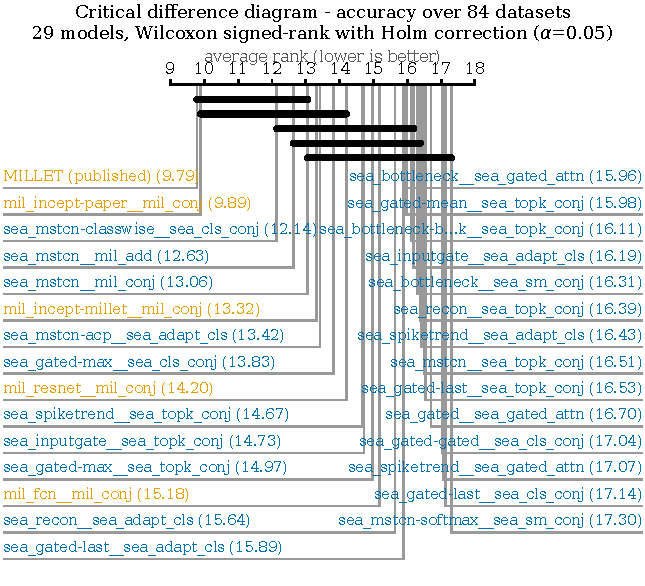
\includegraphics[width=0.85\textwidth]{results/paper_figures/01_main_figures/fig4_critical_difference_accuracy}
  \caption{Critical-difference diagram over the shared \ucr{} datasets. Lower rank is better;
  horizontal bars join models that are not significantly different after Holm correction. Orange
  labels are reproduced baselines, blue are ours. Ranks differ from \Cref{tab:app_ucr} because this
  diagram includes one additional entry --- see the text above.}
  \label{fig:app_cd}
\end{figure}

\subsection{Cost against quality across the whole sweep}
\label{app:pareto}

\begin{figure}[h]
  \centering
  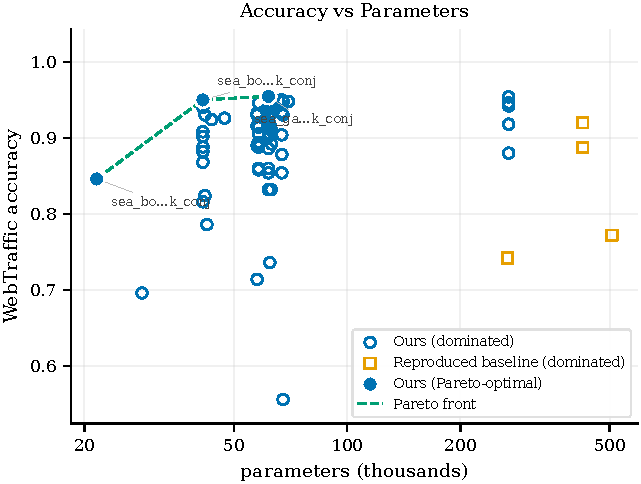
\includegraphics[width=0.6\textwidth]{results/paper_figures/01_main_figures/pareto_web_acc_vs_params}
  \caption{All 72 swept encoder--head combinations (circles) and the reproduced baselines (squares)
  on \webtraffic{}. Filled circles are Pareto-optimal: nothing beats them on both axes at once. The
  baselines occupy the right-hand quarter of the parameter axis without occupying the top of the
  accuracy axis, which is the picture behind \Cref{tab:main,tab:cost}. Labels are abbreviated
  configuration names; \Cref{tab:app_leaderboard} gives them in full.}
  \label{fig:app_pareto}
\end{figure}

\subsection{Relation to published \millet{} results}
\label{app:published}

\begin{table}[h]
\caption{Five ways of obtaining a \millet{} number, and what each is evidence for.}
\label{tab:app_published}
\begin{center}
\small
\begin{tabular}{lcc}
\toprule
\textbf{How obtained} & \webtraffic{} Acc. & \ucr{}-85 Acc. \\
\midrule
Published, mean of 5 seeds \citep{early2024millet} & 0.924 & 0.8445 \\
Published, 5-model ensemble                        & 0.940 & --- \\
Released weights, evaluated in our pipeline        & 0.922 & --- \\
Re-trained here under \emph{their} hyperparameters & 0.920 & 0.8434 \\
Re-trained here under \emph{our} configuration     & 0.887 & 0.8274 \\
\bottomrule
\end{tabular}
\end{center}
\end{table}

The third and fourth rows agree with the first to within $0.4$ and $0.1$ accuracy points, which is
the check that our re-implementation is faithful. The gap between the fourth and fifth rows is
therefore the training budget and nothing else, and it is why the main comparison in \Cref{tab:main}
treats the matched-budget row as the like-for-like baseline while still printing the published-recipe
row as the harder target. We do not reproduce \millet{}'s published AOPCR in this table:
\Cref{sec:res:aopcr} shows it would not be comparable with any value we measured, and quoting it
would contradict our own finding.

\subsection{Full sweep}
\label{app:leaderboard}

\Cref{tab:app_leaderboard} lists all 72 encoder--head combinations, ordered by \webtraffic{}
accuracy. \ucr{} columns are blank where the combination was not run on the archive; those
combinations were screened on \webtraffic{} only, under a fixed compute allocation. One row,
\texttt{seanet\_bottleneck\_adaptive}, completed only 6 of the 85 \ucr{} datasets, so its \ucr{}
values are omitted rather than reported --- a 6-dataset mean is not comparable with an 85-dataset
mean.

% GENERATED by scripts/make_leaderboard_tex.py from
% results/SEA_NET/leaderboard.csv -- do not edit by hand.
{\scriptsize
\setlength{\tabcolsep}{3pt}
\begin{longtable}{rlllcccrr}
\caption{All 72 encoder--head combinations, ordered by \webtraffic{} accuracy. A dash in the
\ucr{} column means the combination was tested on \webtraffic{} only. Pooling heads marked
$^{*}$ are \millet{}'s own, used unchanged.}
\label{tab:app_leaderboard} \\
\toprule
\# & \textbf{Configuration} & \textbf{Encoder} & \textbf{Head} &
Acc. & AOPCR & \ndcg{} & \ucr{}-85 & Params \\
\midrule
\endfirsthead
\multicolumn{9}{l}{\emph{\Cref{tab:app_leaderboard} continued from the previous page.}} \\
\toprule
\# & \textbf{Configuration} & \textbf{Encoder} & \textbf{Head} &
Acc. & AOPCR & \ndcg{} & \ucr{}-85 & Params \\
\midrule
\endhead
\midrule
\multicolumn{9}{r}{\emph{continued on the next page}} \\
\endfoot
\bottomrule
\endlastfoot
1 & \texttt{seanet\_gated\_mean\_topk} & gated & Top-$k$ & 0.955 & 2.23 & 0.750 & 0.8083 & 61{,}740 \\
2 & \texttt{seanet\_conjunctive} & plain & conjunctive* & 0.954 & 1.50 & 0.698 & 0.8238 & 269{,}083 \\
3 & \texttt{seanet\_gated\_max\_topk} & gated & Top-$k$ & 0.952 & 2.27 & 0.719 & 0.8108 & 61{,}740 \\
4 & \texttt{seanet\_topk\_nofocus} & bottleneck & Top-$k$ & 0.950 & 2.30 & 0.765 & --- & 41{,}324 \\
5 & \texttt{seanet\_spiketrend\_topk} & spike/trend & Top-$k$ & 0.950 & 2.32 & 0.756 & 0.8089 & 67{,}020 \\
6 & \texttt{seanet\_inputgate\_mschan} & ms-channels & Top-$k$ & 0.948 & 2.32 & 0.757 & --- & 69{,}768 \\
7 & \texttt{seanet\_gated\_mschan} & ms-channels & Top-$k$ & 0.948 & 2.22 & 0.717 & --- & 67{,}592 \\
8 & \texttt{seanet\_bottleneck\_topk} & bottleneck & Top-$k$ & 0.947 & 2.62 & 0.772 & 0.8097 & 41{,}324 \\
9 & \texttt{seanet\_recon\_adaptive} & recon & adaptive & 0.946 & 2.60 & 0.768 & 0.8140 & 62{,}935 \\
10 & \texttt{seanet\_inputgate\_topk} & input-gated & Top-$k$ & 0.946 & 2.80 & 0.748 & 0.8131 & 58{,}092 \\
11 & \texttt{seanet\_classwise} & plain & class-wise & 0.946 & 1.72 & 0.686 & 0.8292 & 269{,}164 \\
12 & \texttt{seanet\_gated\_max} & gated & class-wise & 0.944 & 1.89 & 0.592 & 0.8237 & 61{,}740 \\
13 & \texttt{seanet\_gated\_last\_topk} & gated & Top-$k$ & 0.942 & 2.31 & 0.748 & 0.8015 & 61{,}740 \\
14 & \texttt{seanet} & plain & additive* & 0.942 & 1.58 & 0.729 & 0.8298 & 269{,}083 \\
15 & \texttt{seanet\_gated\_last} & gated & class-wise & 0.942 & 2.52 & 0.742 & 0.7888 & 61{,}740 \\
16 & \texttt{seanet\_recon\_topk} & recon & Top-$k$ & 0.940 & 2.51 & 0.698 & 0.8063 & 62{,}925 \\
17 & \texttt{seanet\_topk\_k025} & bottleneck & Top-$k$ & 0.940 & 2.65 & 0.733 & --- & 41{,}324 \\
18 & \texttt{seanet\_bottleneck\_softmax} & bottleneck & softmax & 0.940 & 1.68 & 0.740 & 0.8106 & 41{,}325 \\
19 & \texttt{seanet\_gated\_last\_adaptive} & gated & adaptive & 0.938 & 2.39 & 0.793 & 0.8029 & 61{,}750 \\
20 & \texttt{seanet\_spiketrend\_adaptive} & spike/trend & adaptive & 0.934 & 1.91 & 0.747 & 0.8010 & 67{,}030 \\
21 & \texttt{seanet\_recon\_softmax} & recon & softmax & 0.932 & 1.64 & 0.723 & --- & 62{,}926 \\
22 & \texttt{seanet\_slim\_topk} & plain & Top-$k$ & 0.932 & 2.69 & 0.778 & 0.8093 & 57{,}580 \\
23 & \texttt{seanet\_bottleneck\_gatedattn} & bottleneck & gated-attn & 0.930 & 2.23 & 0.741 & 0.8146 & 41{,}844 \\
24 & \texttt{seanet\_spiketrend\_gatedattn} & spike/trend & gated-attn & 0.930 & 1.59 & 0.721 & 0.8039 & 67{,}540 \\
25 & \texttt{seanet\_gated} & gated & class-wise & 0.930 & 2.41 & 0.637 & 0.7900 & 61{,}740 \\
26 & \texttt{seanet\_slim\_adaptive} & plain & adaptive & 0.930 & 2.45 & 0.793 & --- & 57{,}590 \\
27 & \texttt{seanet\_bottleneck\_mschan} & ms-channels & Top-$k$ & 0.926 & 2.24 & 0.777 & --- & 47{,}176 \\
28 & \texttt{seanet\_bottleneck\_mschan\_lean} & ms-channels & Top-$k$ & 0.924 & 2.76 & 0.735 & --- & 43{,}576 \\
29 & \texttt{seanet\_gated\_last\_softmax} & gated & softmax & 0.920 & 1.99 & 0.738 & --- & 61{,}741 \\
30 & \texttt{millet\_paper} & InceptionTime & conjunctive* & 0.920 & 13.27 & 0.661 & 0.8434 & 423{,}707 \\
31 & \texttt{seanet\_acp} & plain & adaptive & 0.918 & 1.61 & 0.619 & 0.8134 & 269{,}174 \\
32 & \texttt{seanet\_gated\_last\_gatedattn} & gated & gated-attn & 0.918 & 1.35 & 0.757 & 0.8048 & 62{,}260 \\
33 & \texttt{seanet\_slim} & plain & class-wise & 0.916 & 2.48 & 0.719 & --- & 57{,}580 \\
34 & \texttt{seanet\_gated\_max\_softmax} & gated & softmax & 0.914 & 1.88 & 0.776 & --- & 61{,}741 \\
35 & \texttt{seanet\_inputgate} & input-gated & class-wise & 0.914 & 2.48 & 0.715 & --- & 58{,}092 \\
36 & \texttt{seanet\_gated\_mean\_softmax} & gated & softmax & 0.912 & 2.09 & 0.765 & --- & 61{,}741 \\
37 & \texttt{seanet\_recon} & recon & class-wise & 0.910 & 2.50 & 0.680 & --- & 62{,}925 \\
38 & \texttt{seanet\_topk\_k100} & bottleneck & Top-$k$ & 0.908 & 2.44 & 0.722 & --- & 41{,}324 \\
39 & \texttt{seanet\_gated\_max\_adaptive} & gated & adaptive & 0.906 & 2.07 & 0.729 & --- & 61{,}750 \\
40 & \texttt{seanet\_inputgate\_adaptive} & input-gated & adaptive & 0.905 & 2.65 & 0.732 & 0.8153 & 58{,}102 \\
41 & \texttt{seanet\_spiketrend} & spike/trend & class-wise & 0.904 & 2.15 & 0.699 & --- & 67{,}020 \\
42 & \texttt{seanet\_bottleneck} & bottleneck & class-wise & 0.902 & 2.57 & 0.733 & --- & 41{,}324 \\
43 & \texttt{seanet\_gated\_mean} & gated & class-wise & 0.902 & 2.49 & 0.714 & --- & 61{,}740 \\
44 & \texttt{seanet\_inputgate\_softmax} & input-gated & softmax & 0.894 & 1.64 & 0.696 & --- & 58{,}093 \\
45 & \texttt{seanet\_slim\_gatedattn} & plain & gated-attn & 0.894 & 2.30 & 0.714 & --- & 58{,}100 \\
46 & \texttt{seanet\_recon\_attnmax} & recon & attn-max & 0.892 & 2.32 & 0.725 & --- & 62{,}935 \\
47 & \texttt{seanet\_slim\_softmax} & plain & softmax & 0.890 & 1.83 & 0.705 & --- & 57{,}581 \\
48 & \texttt{seanet\_slim\_gatedattn} & gated & attention* & 0.888 & 2.40 & 0.710 & --- & 58{,}100 \\
49 & \texttt{seanet\_topk\_k005} & bottleneck & Top-$k$ & 0.888 & 2.29 & 0.715 & --- & 41{,}324 \\
50 & \texttt{millet} & InceptionTime & conjunctive* & 0.887 & 2.57 & 0.677 & 0.8274 & 423{,}707 \\
51 & \texttt{seanet\_gated\_max\_attnmax} & gated & attn-max & 0.886 & 1.12 & 0.575 & --- & 61{,}750 \\
52 & \texttt{seanet\_topk\_k050} & bottleneck & Top-$k$ & 0.882 & 3.11 & 0.732 & --- & 41{,}324 \\
53 & \texttt{seanet\_softmax} & plain & softmax & 0.880 & 1.02 & 0.605 & 0.8131 & 269{,}165 \\
54 & \texttt{seanet\_spiketrend\_softmax} & spike/trend & softmax & 0.878 & 1.43 & 0.665 & --- & 67{,}021 \\
55 & \texttt{seanet\_bottleneck\_adaptive} & bottleneck & adaptive & 0.868 & 1.97 & 0.680 & --- & 41{,}334 \\
56 & \texttt{seanet\_slim\_dualstream} & plain & dual-stream & 0.860 & 2.40 & 0.745 & --- & 58{,}101 \\
57 & \texttt{seanet\_gated\_mean\_adaptive} & gated & adaptive & 0.860 & 2.24 & 0.731 & --- & 61{,}750 \\
58 & \texttt{seanet\_inputgate\_attnmax} & input-gated & attn-max & 0.858 & 2.15 & 0.700 & --- & 58{,}102 \\
59 & \texttt{seanet\_spiketrend\_attnmax} & spike/trend & attn-max & 0.854 & 1.65 & 0.644 & --- & 67{,}030 \\
60 & \texttt{seanet\_gated\_last\_attnmax} & gated & attn-max & 0.854 & 1.78 & 0.668 & --- & 61{,}750 \\
61 & \texttt{seanet\_bottleneck\_shallow} & bottleneck & Top-$k$ & 0.846 & 2.82 & 0.624 & --- & 21{,}548 \\
62 & \texttt{seanet\_gated\_mean\_attnmax} & gated & attn-max & 0.832 & 1.67 & 0.704 & --- & 61{,}750 \\
63 & \texttt{seanet\_gated\_pyramid} & ms-pyramid & Top-$k$ & 0.832 & 0.98 & 0.591 & --- & 62{,}781 \\
64 & \texttt{seanet\_bottleneck\_dualstream} & bottleneck & dual-stream & 0.824 & 2.04 & 0.652 & --- & 41{,}845 \\
65 & \texttt{seanet\_bottleneck\_attnmax} & bottleneck & attn-max & 0.816 & 1.74 & 0.610 & --- & 41{,}334 \\
66 & \texttt{seanet\_bottleneck\_pyramid} & ms-pyramid & Top-$k$ & 0.786 & 1.03 & 0.569 & --- & 42{,}365 \\
67 & \texttt{resnet} & ResNet & conjunctive* & 0.772 & 2.95 & 0.554 & 0.8146 & 506{,}331 \\
68 & \texttt{fcn} & FCN & conjunctive* & 0.742 & 3.83 & 0.533 & 0.8141 & 267{,}035 \\
69 & \texttt{seanet\_gated\_last\_dualstream} & gated & dual-stream & 0.736 & 1.95 & 0.637 & --- & 62{,}261 \\
70 & \texttt{seanet\_slim\_attnmax} & plain & attn-max & 0.714 & 1.63 & 0.532 & --- & 57{,}590 \\
71 & \texttt{seanet\_bottleneck\_mschan\_pyramid} & ms-pyramid & Top-$k$ & 0.696 & 2.17 & 0.653 & --- & 28{,}441 \\
72 & \texttt{seanet\_spiketrend\_dualstream} & spike/trend & dual-stream & 0.556 & 1.64 & 0.510 & --- & 67{,}541 \\
\end{longtable}}

